\documentclass[a4paper]{article}
\usepackage[a4paper,top=2cm,bottom=2cm,left=1cm,right=1cm,marginparwidth=1.75cm]{geometry}
% \usepackage[spanish]{babel}
% \selectlanguage{spanish}
% \usepackage[utf8]{inputenc}
% \usepackage[T1]{fontenc}
% \usepackage[spanish]{babel}

% \usepackage[T1]{fontenc}
\usepackage{graphicx} %Paquete para usar imagenes
\usepackage{listings}
\usepackage{xcolor}
\usepackage{tcolorbox}

\definecolor{background}{HTML}{E7EBF4}
\definecolor{bg}{HTML}{1a1b26}
\definecolor{fg}{HTML}{a9b1d6}
\definecolor{comment}{HTML}{848cb5}
\definecolor{cyan}{HTML}{82aaff}
\definecolor{orange}{HTML}{ff9e64}
\definecolor{yellow}{HTML}{e9d78e}
\definecolor{purple}{HTML}{c792ea}
\definecolor{green}{HTML}{7fdbca}
\definecolor{numbers}{HTML}{9854f1}
\definecolor{keyword}{HTML}{9854f1}

\lstset{
    showspaces=false, % Evita mostrar espacios en blanco como ␣
    showstringspaces=false,
    inputencoding=utf8,
    extendedchars=true,
    literate=%
    {á}{{\'a}}1
    {é}{{\'e}}1
    {í}{{\'i}}1
    {ó}{{\'o}}1
    {ú}{{\'u}}1
    {ñ}{{\~n}}1
}
\lstdefinestyle{mystyle}{
    language=Python,
    basicstyle=\ttfamily,
    keywordstyle=\color{keyword},
    commentstyle=\color{comment},
    numbers=none,
    numberstyle=\tiny\color{numbers},
    frame=none,
    breaklines=true,
    % showstringspaces=false
    xleftmargin=0mm,
    xrightmargin=0mm,
}

\lstset{style=mystyle}

\newtcolorbox{mycodebox}[1][]{
    arc=17pt,  % Radio de las esquinas redondeadas
    colback=background,  % Color de fondo del cuadro
    boxrule=0.5pt,  % Grosor de la línea del cuadro
    colframe=background,
    width=0.8\textwidth,   % Anchura del cuadro
    % height=5cm,            % Altura del cuadro
    % breakable,
    #1  % Otras opciones personalizadas que puedas necesitar
}


\newtcolorbox{mycodeboxl}[1][]{
    arc=7pt,  % Radio de las esquinas redondeadas
    colback=background,  % Color de fondo del cuadro
    boxrule=0.5pt,  % Grosor de la línea del cuadro
    colframe=background,
    width=0.94\textwidth,   % Anchura del cuadro
    % height=5cm,            % Altura del cuadro
    % breakable,
    #1  % Otras opciones personalizadas que puedas necesitar
}

% Documento
\begin{document}
\newgeometry{left=3cm,right=3cm,top=2cm,bottom=2cm}
\begin{titlepage}

%--------------- Nuevo comendo de linea ----------------->
\newcommand{\linea}{\rule{\linewidth}{0.7mm}} 
\center
%--------------- Universidad, facultad y carrera ----------------->
\textbf{\Large UNIVERSIDAD NACIONAL DE SAN ANTONIO ABAD DEL CUSCO}\\[0.2cm]
\textbf{\Large FACULTAD DE INGENIERÍA ELÉCTRICA, ELECTRÓNICA,INFORMÁTICA Y MECÁNICA}\\[0.2cm]
\textbf{\Large INGENIERÍA INFORMÁTICA Y DE SISTEMAS\\[0.6cm]}

%--------------- Escudos png ----------------->

\includegraphics[width=8cm]{src/escudo-unsaac.png}
\vfill

%--------------- Tema ----------------->
\linea
\\[0.3cm]
% \vfill
\textbf{\LARGE Guía de Laboratorio 7 - Deformación 2D}\\[0.2cm]
\linea \\
\vfill

%--------------- Integrantes ----------------->
\textit{\Large Alumno:}\\
%Integrantes del grupo
    \textbf{\large Ian Logan Will Quispe Ventura}\\
    \textit{211359}\\
    % \vfill

%--------------- Profesor y curso ----------------->
\vspace{0.3cm}
    \textit{\Large Docente:}\\
    \textbf{\large Hector Eduardo Ugarte Rojas}\\
\vspace{0.5cm}
    \textit{\Large Curso:}\\
    \textbf{\large Computación Gráfica}\\
    \vfill

\vspace{0.4cm}
    \textbf{\Large Cusco - Perú }\\
    \textbf{\large 2023 - II }\\
    \newpage
    \end{titlepage}

\restoregeometry
\newpage
% •·•·•·•·•·•••·•·•·•·•·•·•·•·•·•·•·•·•·•·•·•·•·•·•·•·•.,..,
% \section{Funcionamiento del algoritmo DDA}

\Large{\textbf{Deformación de un rectángulo en el eje X}}\\[-0.4cm]
\begin{center}
\begin{mycodeboxl}
\begin{lstlisting}
from OpenGL.GL import *
from OpenGL.GLU import *
from OpenGL.GLUT import *
 
# Deformación de rectángulo con respecto al eje X
def deformaRectanguloX(x1, y1, x2, y2, sh):
 
    #--dibujar el rectangulo original
    glColor3f (0.5 , 0.3 , 0.9) # Color1
    glBegin(GL_LINE_LOOP)
    glVertex2f(x1, y1)
    glVertex2f(x2, y1)
    glVertex2f(x2, y2)
    glVertex2f(x1, y2)
    glEnd()
    # Deformar cada punto del rectangulo con respecto al eje X
    x1d = x1 + sh * y1
    y1d = y1
    x2d = x2 + sh * y1
    y2d = y1
 
    x3d = x2 + sh * y2
    y3d = y2
    x4d = x1 + sh * y2
    y4d = y2
    # Dibujar el rectangulo deformado con respecto al eje X
    glColor3f(0.8, 0.26, 1.0) # Color2
    glBegin(GL_LINE_LOOP)
    glVertex2f(x1d, y1d)
    glVertex2f(x2d, y2d)
    glVertex2f(x3d, y3d)
    glVertex2f(x4d, y4d)
    glEnd()
\end{lstlisting}
\end{mycodeboxl}
\end{center}
% -------------------------------------------------------------------
\newpage
\begin{center}
\begin{mycodeboxl}
\begin{lstlisting}
#--despliega el gráfico
def display():
    x1 = 20.0
    y1 = 50.0
    x2 = 250.0
    y2 = 200.0
    sh = 2
    glClear(GL_COLOR_BUFFER_BIT) 
    deformaRectanguloX(x1, y1, x2, y2, sh)
    glFlush() 

def myinit():
    glClearColor (0.9 ,0.92 , 0.95 , 1.0) # Fondo
    glPointSize(1.0) #--tamño de los puntos
    glMatrixMode(GL_PROJECTION)
    glLoadIdentity()
    gluOrtho2D(0.0, 659.0, 0.0, 299.0)
 
def main():
    glutInit(sys.argv)
    glutInitDisplayMode(GLUT_SINGLE | GLUT_RGB)
    glutInitWindowSize(500, 500)
    glutInitWindowPosition(0, 0)
    glutCreateWindow("Reflexión")
    glutDisplayFunc(display)
    myinit() # fija 
    glutMainLoop() 
 
if __name__ == "__main__":
    main()
\end{lstlisting}
\end{mycodeboxl}
\end{center}
\newpage
% -------------------------------------------------------------------
Gráfico generado 
\begin{center}
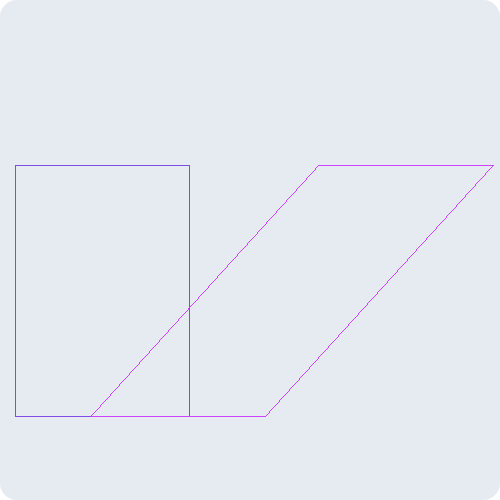
\includegraphics[width=16cm]{src/1.png}
\end{center}
\newpage
\Large{\textbf{Deformación de un rectángulo en el eje Y}}\\[-0.4cm]
\begin{center}
\begin{mycodeboxl}
\begin{lstlisting}
from OpenGL.GL import *
from OpenGL.GLU import *
from OpenGL.GLUT import *
import sys
 
#--deformación de rectángulo con respecto al eje X
def deformaRectanguloX(x1, y1, x2, y2, sh):
    #Dibujar el rectangulo original
    glColor3f (0.5 , 0.3 , 0.9) # Color1
    glBegin(GL_LINE_LOOP)
    glVertex2f(x1, y1)
    glVertex2f(x2, y1)
    glVertex2f(x2, y2)
    glVertex2f(x1, y2)
    glEnd()
    # Deformar cada punto del rectangulo con respecto al eje X
    x1d = x1 
    y1d = y1 + sh * x1
    x2d = x2 
    y2d = y1 + sh * x2
 
    x3d = x2 
    y3d = y2 + sh * x2
    x4d = x1 
    y4d = y2 + sh * x1
    # Dibujar el rectangulo deformado con respecto al eje X
    glColor3f(0.8, 0.26, 1.0) # Color2
    glBegin(GL_LINE_LOOP)
    glVertex2f(x1d, y1d)
    glVertex2f(x2d, y2d)
    glVertex2f(x3d, y3d)
    glVertex2f(x4d, y4d)
    glEnd()
\end{lstlisting}
\end{mycodeboxl}
\end{center}
% -------------------------------------------------------------------

\begin{center}
\begin{mycodebox}
\begin{lstlisting}
#--despliega el gráfico
def display():
    x1 = 20.0
    y1 = 50.0
    x2 = 230.0
    y2 = 200.0
    sh = 2
    glClear(GL_COLOR_BUFFER_BIT)
    deformaRectanguloX(x1, y1, x2, y2, sh)
    glFlush()
 
def myinit():
    glClearColor (0.9 ,0.92 , 0.95 , 1.0) # Fondo
    glPointSize(1.0) 
    glMatrixMode(GL_PROJECTION)
    glLoadIdentity()
    gluOrtho2D(0.0, 260.0, 0.0, 670.0)
 
def main():
    glutInit(sys.argv)
    glutInitDisplayMode(GLUT_SINGLE | GLUT_RGB)
    glutInitWindowSize(500, 500) 
    glutInitWindowPosition(0, 0)
    glutCreateWindow("Reflexión")
    glutDisplayFunc(display)
    myinit() 
    glutMainLoop()
 
if __name__ == "__main__":
    main()
\end{lstlisting}
\end{mycodebox}
\end{center}
% -------------------------------------------------------------------
\newpage
Gráfico generado\\
\begin{center}
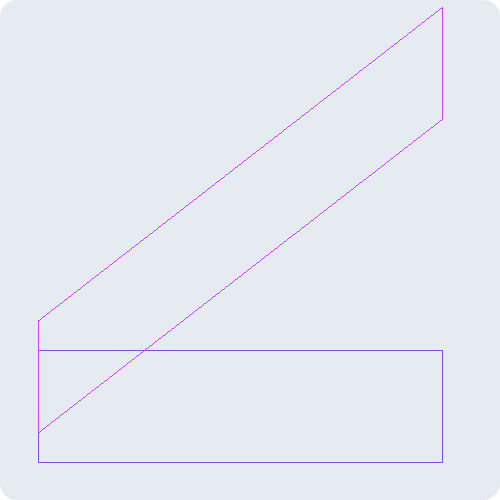
\includegraphics[width=16cm]{src/2.png}
\end{center}
\newpage


\Large{\textbf{Deformación de "E" en el eje X}}\\[-0.4cm]
\begin{center}
\begin{mycodeboxl}
\begin{lstlisting}
from OpenGL.GL import *
from OpenGL.GLU import *
from OpenGL.GLUT import *
import sys
 
# Matriz de coordenadas del dibujo original
matriz_origen = [[200, 300, 300, 300, 300, 280, 200, 280],
[200, 290, 230, 290, 230, 180, 200, 180],
[200, 250, 260, 250, 260, 230, 200, 230],
[200, 200, 300, 200, 300, 180, 200, 180]]
 
# Dibujar la figura original
def dibujar_E():
    glBegin(GL_QUADS)
    glColor3f (0.5 , 0.3 , 0.9) # Color1
    for i in range(4):
        for j in range(0, 8, 2):
            glVertex2f(matriz_origen[i][j], matriz_origen[i][j+1])
    glEnd()
 
# Algoritmo de deformación
def deformaPuntoX(x, y, sh):
    return x + sh * y, y
 
# Dibuajar la figura E deformada respecto a x
def dibujar_E_deformado(sh):
    glBegin(GL_QUADS)
    glColor3f(0.8, 0.26, 1.0) # Color2
    for i in range(4):
        for j in range(0, 8, 2):
            x, y = deformaPuntoX(matriz_origen[i][j], matriz_origen[i][j+1], sh)
            glVertex2f(x, y)
    glEnd()
\end{lstlisting}
\end{mycodeboxl}
\end{center}
% -------------------------------------------------------------------
\newpage

\begin{center}
\begin{mycodeboxl}
\begin{lstlisting}
def display():
    glClear(GL_COLOR_BUFFER_BIT) 
    dibujar_E()
    dibujar_E_deformado(2)
    glFlush() 
def display():
    glClear(GL_COLOR_BUFFER_BIT) 
    dibujar_E()
    dibujar_E_deformado(2)
    glFlush() 
 
def myinit():
    glClearColor (0.9 ,0.92 , 0.95 , 1.0)
    glPointSize(1.0)
    glMatrixMode(GL_PROJECTION)
    glLoadIdentity()
    gluOrtho2D(0.0, 999.0, 0.0, 499.0)
 
def main():
    glutInit(sys.argv)
    glutInitDisplayMode(GLUT_SINGLE | GLUT_RGB)
    glutInitWindowSize(500, 500)
    glutInitWindowPosition(0, 0)
    glutCreateWindow("Reflexión") 
    glutDisplayFunc(display)
    myinit()
    glutMainLoop()
 
if __name__ == "__main__":
    main()
\end{lstlisting}
\end{mycodeboxl}
\end{center}
\newpage
Gráfico generado\\
\begin{center}

\includegraphics[width=16cm]{src/3.png}
\end{center}
\newpage
% -------------------------------------------------------------------
\Large{\textbf{Deformación de "E" en el eje Y}}\\[-0.4cm]
\begin{center}
\begin{mycodeboxl}
\begin{lstlisting}
from OpenGL.GL import *
from OpenGL.GLU import *
from OpenGL.GLUT import *
import sys
 
# Matriz de coordenadas del dibujo original
matriz_origen = [[200, 300, 300, 300, 300, 280, 200, 280],
[200, 290, 230, 290, 230, 180, 200, 180],
[200, 250, 260, 250, 260, 230, 200, 230],
[200, 200, 300, 200, 300, 180, 200, 180]]
 
# Dibujar la figura original
def dibujar_E():
    glBegin(GL_QUADS)
    glColor3f (0.5 , 0.3 , 0.9) # Color1
    for i in range(4):
        for j in range(0, 8, 2):
            glVertex2f(matriz_origen[i][j], matriz_origen[i][j+1])
    glEnd()
 
# Algoritmo de deformación
def deformaPuntoY(x, y, sh):
    return y + sh * x, x
 
# Dibujar la figura E deformada respecto a y
def dibujar_E_deformado(sh):
    glBegin(GL_QUADS)
    glColor3f(0.8, 0.26, 1.0) # Color2
    for i in range(4):
        for j in range(0, 8, 2):
            x, y = deformaPuntoY(matriz_origen[i][j], matriz_origen[i][j+1], sh)
            glVertex2f(x, y)
    glEnd()
\end{lstlisting}
\end{mycodeboxl}
\end{center}
\newpage
\begin{center}
\begin{mycodebox}
\begin{lstlisting}
 
def display():
    glClear(GL_COLOR_BUFFER_BIT)
    dibujar_E()
    dibujar_E_deformado(2)
    glFlush()
  def myinit():
    glClearColor (0.9 ,0.92 , 0.95 , 1.0) # Fondo
    glPointSize(1.0) 
    glMatrixMode(GL_PROJECTION)
    glLoadIdentity()
    gluOrtho2D(0.0, 999.0, 0.0, 499.0)
 
def main():
    glutInit(sys.argv)
    glutInitDisplayMode(GLUT_SINGLE | GLUT_RGB)
    glutInitWindowSize(500, 500) 
    glutInitWindowPosition(0, 0)
    glutCreateWindow("Reflexión") 
    glutDisplayFunc(display)
    myinit() 
    glutMainLoop()
 
if __name__ == "__main__":
    main()
\end{lstlisting}
\end{mycodebox}
\end{center}
\newpage
Gráfico generado\\
\begin{center}

\includegraphics[width=16cm]{src/4.png}
\end{center}
\end{document}
